\subsection{Jet reconstruction with the anti-$k_{t}$ algorithm}

The goal in jet reconstruction is to identify clusters of hadrons originating from a fragmenting high-energy parton.  In high-$p_{\rm T}$ jet studies in pp collisions, the general locations of jets in an event may be qualitatively obvious via large energy deposits in calorimeters;  however, there is no clear single standard of how jet boundaries should be drawn.  In practice, jets are defined by the algorithms used to find and determine their direction.  These algorithms fall in two primary categories:  ``cone algorithms,'' which define jets within specific conical regions (based on the fact that hadronization has little effect total momentum flow), and ``sequential recombination algorithms,'' which iteratively identify and cluster pairs of closest particles to form jets that are not necessarily conical.~\cite{Salam:2009jx, bib_antikt, Cacciari:fastjet1}.  Several properties are desireable, from theoretical and experimental perspectives, in jet finding: 
\begin{itemize}
\item Straightforward implementation for both theoretical calculations and jet-finding and reconstruction in experimental measurements
\item Cross-sections that are finite in perturbation theory
\item Infrared and collinear (IRC) safety -- the property that a soft collinear emission in a parton splitting should not modify the overall collection of hard (high-$p_{\rm T}$) jets in the event, in particular avoiding the possibility of non-cancelling divergences in perturbation calculations
\item Soft resilience -- clustering jets that are reasonably regular and not overly sensitive to soft particles, a property motivated by the finite resolution of experimental detectors.
\end{itemize}

\noindent Heavy ion jet studies in CMS use the anti-$k_{t}$ algorithm, a soft-resilent, IRC safe, and straightforward sequential recombination algorithm~\cite{bib_antikt}, implemented in the FastJet framework~\cite{Cacciari:fastjet1}.  The anti-$k_{t}$ algorithm clusters entities (calorimeter towers, particles, or partially clustered pseudo-jets) $i$ and $j$ based on the distance measures $d_{ij}$ between the two particles and $d_{iB}$ between the particle and beam, with the measures defined as: 

\begin{equation}
\label{eq:a_kt1}
d_{ij} = {\rm min}(k_{ti}^{-2},k_{tj}^{-2})\frac{(\Delta R_{ij})^{2}}{R^{2}}, 
\end{equation}

\begin{equation}
\label{eq:a_kt2}
d_{iB} = k_{ti}^{-2},
\end{equation}

\noindent where $k_{ti}$ refers to the transverse momentum of particle $i$, $\Delta R_{ij}$ refers to the spatial distance (in rapidity and azimuth) between the two particles, and radius parameter $R$ is a reconstruction parameter.  The name anti-$k_{t}$ derives from the negative exponent for $k_{t}$ (in contrast to other sequential recombination algorithms), which enables IRC safety and soft resilience by making jet shape sensitivity to a particle inversely correlated to the particle's transverse momentum.  With this low sensitivity to soft particles, the anti-$k_{t}$ algorithm results in a collection of mostly circular jets (except in the case of jets separated by less than $2R$, in which each jet has a radius of $\pi R^{2}$.  The choice of parameter $R$ is a trade-off between capturing more fragmentation products (as can extend as far as $\Delta R{ij}$ = 0.8 in pp collisions), and limiting the influence of background particles in jet reconstruction.  In heavy ion experimental studies, where background levels are very high, typical choices of R range from 0.2 to 0.5.  

With the CMS detector, jets may be clustered from ECAL and HCAL information only (``calorimeter jets'') or from information from the full detector, using the particle flow (PF) algorithm.  The PF algorithm improves jet energy resolution (JER) substantially at low-$p_{\rm T}$ (at 10 GeV JER is 15\% for PF jets versus 40\% for calorimeter jets) with improvements decreasing for higher-$p_{\rm T}$ jets (at 100 GeV PF jet JER is 8\% versus 12\% for calorimeter jets, falling to a difference of 4\% versus 5\% at 1 TeV).  For jet-track correlation studies, however, the resolution improvements that the particle flow algorithm offers come at the cost of enhancing sensitivity to tracking biases in the jet-track correlation signal, since low-$p_{\rm T}$ tracks are included in jet reconstruction.  In this analysis, calorimeter jets are used to avoid these auto-correlation effects, and because we will consider jets with $p_{\rm T} > 120$ GeV for which calorimeter jet energy resolution is adequate.  Jets are reconstructed with anti-$k_{t}$ radius $R = 0.3$ for 2.76 TeV data (``ak3Calo'' jets), and with radius $R = 0.4$ for 5.02 TeV data (``ak4Calo'' jets).  In pp data at 2.76 TeV and 5.02 TeV the contribution to the jet energy from the underlying event (UE) is negligible (less than 1 GeV), so no underlying event subtraction is employed.
 
 
\subsection{Underlying event subtraction in PbPb data}

In PbPb collisions it is necessary to subtract contributions from the large underlying event in order to recover the true jet energy.  There are a variety of methods used for underlying event subtraction, of which the following two are relevant for this anlaysis.  

\subsubsection{Noise/pedestal subtraction}
 In most CMS high-$p_{\rm T}$ jet analyses, including 5.02 TeV PbPb data studies here, underlying event subtraction is performed using a variant of an iterative noise/pedestal subtraction technique~\cite{Kodolova:2007hd}.  This algorithm occurs in the following steps: 
 \begin{itemize}
 \item First, the mean ``pedestal'' energy in calorimeter cells as a function of energy $\eta$ ($P(\eta)$) is calculated along with its dispersion.  
 \item The pedestal function $P(\eta)$ is subtracted from all cells.  
 \item Cells with non-physical negative energy entries are then set to zero.
 \item $ \langle{\rm E_{cell}}\rangle + \langle\sigma (\rm E_{cell})\rangle$ is subtracted from each cell to compensate for the elimination of negative energy cells.
 \item Jets are clustered from the pedestal-subtracted cells using the anti-$k_{t}$ algorithm.  
 \item The pedestal function $P(\eta)$ is then re-derived using only cells that are not a part of clustered jets, and the algorithm is repeated.  
 \end{itemize}
 
 \noindent  After this underlying event subtraction is applied, the anti-$k_{t}$ algorithm with radius parameter $R = 0.4$ is then employed for jet reconstruction (``akPu4Calo jets'').  

\subsubsection{HF/Voronoi subtraction}
For 2.76 TeV PbPb data a different algorithm, designed to eliminate the threshold and possible resulting bias from the noise/pedestal technique, is employed~\cite{AN_2014_024}.  This algorithm uses information from the HF detector to model and subtract the underlying event using Voronoi decomposition (``HF/Voronoi'' algorithm) in the following steps: 
\begin{itemize}
\item The distribution of underyling $E_{\rm T}$ as a function of $\eta$ and $\phi$ is modeled using singular value decomposition (SVD) training (${\rm d}p_{\rm T}/{\rm d}\eta / {\rm }\phi$ with Voronoi parameters $v_{1}...v_{4}$) to extrapolate the UE distribution from the HF calorimeter at large $\eta$ to the central analysis region ($|\eta| < 1.6$).
\item The modeled UE distribution is subtracted from all calorimeter cells.
\item Each calorimeter cell is associated with its nearest neighbors, and energy is redistributed between neighboring in an ``equalization'' procedure used to eliminate non-physical negative $E_{\rm T}$ entries (optimized to minimize energy transfers.
\end{itemize}

\noindent After Voronoi subtraction and equalization, the anti-$k_{t}$ algorithm is employed with radius parameter $R = 0.3$ to cluster (``akVs3Calo") jets.

\subsection{Jet energy corrections}
\label{sec:JEC}

Jet reconstruction as described above gives spatial coordinates and $p_{\rm T}$ for each jet as measured by the detector.  Our goal in jet studies, however, is to reconstruct the true total parton or particle energy.  This is achieved through jet energy corrections (JEC) that establish a mapping between measured energy (which does not, for example, include neutrinos produced in jet fragmentation) and ``true'' jet energies.  This mapping is complicated by nonlinearity in detector response.  Initial corrections are derived as a function of $p_{\rm T}$ and $\eta$ using dijet QCD samples of {\sc pythia} and {\sc pythia+hydjet} Monte Carlo, spatially matching reconstructed jets to generated particles, and comparing generated versus reconstructed jet energy for these matched jets.  These ``MC truth'' corrections are applied to measured jet energies to return a collection of jets that, on average, capture the kinematic distribution of the partons before fragmentation.

These corrections do not, however, fully account for the non-linearity of calorimeter response.  In particular, in an effect particularly relevant for jet-track correlation studies, the jet energy scale depends on jet fragmenation.  Given two jets with identical parton energy, the jet with softer fragmentation (i.e. jets with a higher fraction low-$p_{\rm T}$ particles) will be on average reconstructed with lower energy than the jet with harder fragmentation.  When combined wtih a jet selection threshold, this non-linearity results in a bias that systematically underestimates the jets with soft fragmentation in the analysis sample.  An additional fragmentation-function dependent jet energy correction (JFF-JEC) is therefore applied after initial jet energy corrections in order to reduce this bias (detailed in Ref.~\cite{AN_2014_024}).  These JFF-JEC are derived using the number of particle flow candidates ($N_{\rm PF}$) in the jet with $p_{\rm T} > 2$ GeV, with this threshold chosen to reduce the influence of soft fluctuations in the underlying event.   Correction tables are derived as a function of $N_{\rm PF}$, jet $p_{\rm T}$, and PbPb event centrality in {\sc pythia} and {\sc pythia+hydjet} simulation, and are applied to jets after the JECs described above.  Finally, iterative residual corrections are applied as a function of jet $p_{\rm T}$.  The application of JFF-JECs reduces the overall quark/gluon non-closure, as illustrated for PbPb data in Fig.~\ref{fig:quark_gluon}, and slightly improves jet energy resolution overall.

\begin{figure}[hbtp]
\begin{center}
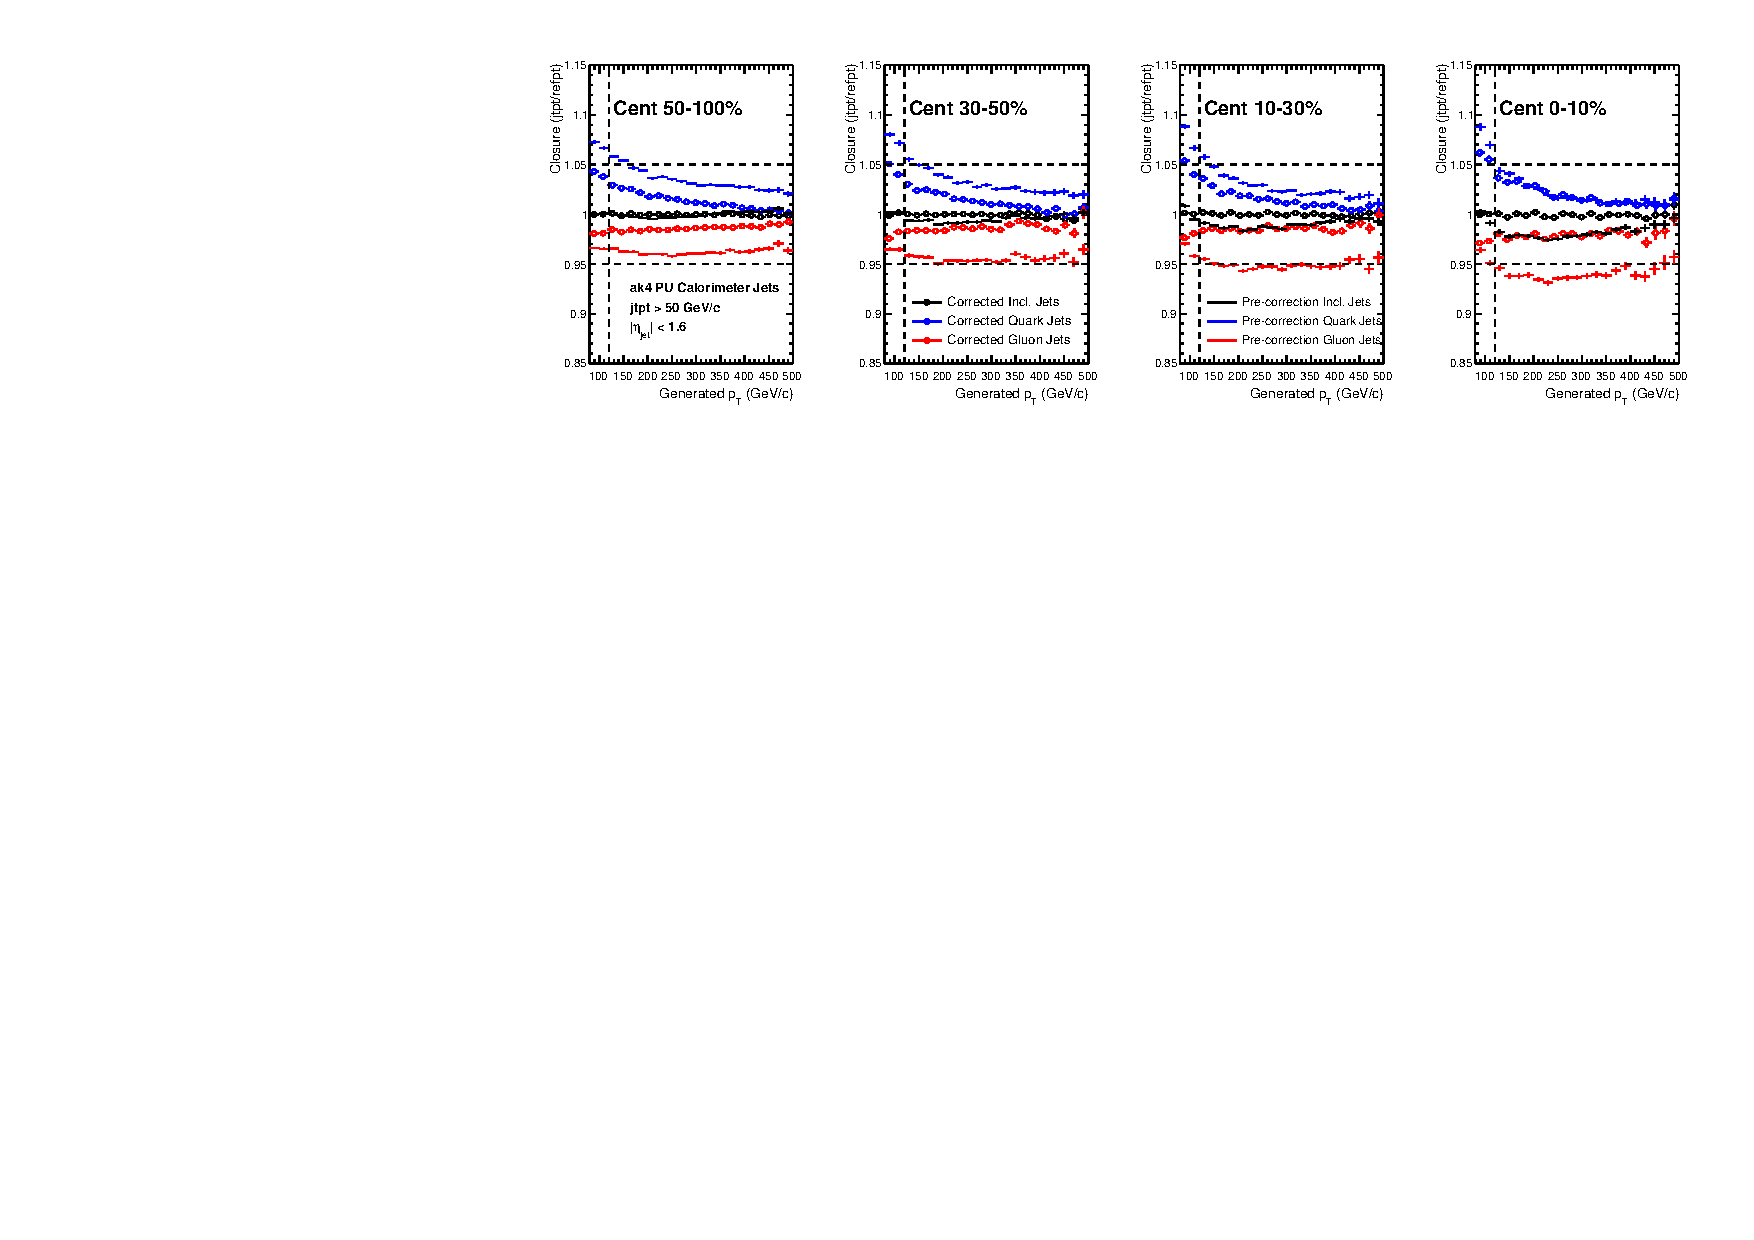
\includegraphics[width=0.99\textwidth]{figures/Detector/fullClosures_DogaIterative_centDep_correctToJetPt.pdf}
\caption{Closure with and without JFF-JEC for quark and gluon jets.}
\label{fig:quark_gluon}
\end{center}
\end{figure}


